\section{Analysis}

\begin{definition}[Entropic Growth]
  The \emph{Entropic Growth} property of
  a \poem execution,
  parametrized by the growth interval $s \in \mathbb{N}$
  and the growth velocity $\tau \in \mathbb{R}^+$,
  states that for
  all honest parties $P$ and all rounds $r_1 + s \leq r_2$,
  the chains $C_1, C_2$ of $P$ at rounds $r_1, r_2$ respectively
  satisfy $\work(C_2[{|C_1|}{:}]) \geq s \tau \lg T$.
\end{definition}

\begin{definition}[Entropic Quality]
  The \emph{Entropic Quality} property of
  a \poem execution, parametrized by the \emph{quality chunk parameter} $\ell \in \mathbb{N}$
  and \emph{quality concentration parameter} $\mu \in \mathbb{R}^+$
  (with $\ell \mu \geq 1$)
  states that for
  all honest parties $P$ and all rounds $r$,
  the chain $C$ of $P$ at round $r$
  has the property that
  for every $0 \leq \alpha < \work(C) - \ell \lg T$,
  there is at least one honestly generated block in the chain
  $[{\alpha}{:}{\alpha + \ell \lg T}] \lhd C$.
\end{definition}

\begin{definition}[Entropic Common Prefix]
  The \emph{Entropic Common Prefix} property of
  a \poem execution, parametrized by the \emph{common prefix parameter} $k \in \mathbb{N}$
  states that for
  all honest parties $P_1, P_2$
  and all rounds $r_1 \leq r_2$,
  the chains $C_1, C_2$ of $P_1, P_2$ at rounds $r_1, r_2$ respectively
  satisfy $[{:}{-k}] \lhd C_1 \preceq C_2$.
\end{definition}

\begin{conjecture}[Entropic Growth]
  Typical executions of \poem satisfy the Entropic Growth property
  with $s = \lambda$ and $\tau = (1 - \epsilon)f$.
\end{conjecture}

\begin{conjecture}[Entropic Quality]
  Typical executions of \poem satisfy the Entropic Quality property
  with $\ell = 2 \lambda f$ and
  $\mu = 1 - (1 + \frac{\delta}{2})\frac{t}{n - t} - \frac{\epsilon}{1 - \epsilon}$.
\end{conjecture}

\begin{conjecture}[Entropic Common Prefix]
  Typical executions of \poem satisfy the Entropic Common Prefix property
  with $k = 2 \lambda f$.
\end{conjecture}

In the analysis we are going to assume honest majority.

\begin{definition}[Honest Majority Assumption]
  A number of $t$ out of $n$ parties are corrupted such that $t \leq (1 - \delta) (n - t)$.
\end{definition}
\atnote{Introduce $3f + 3\epsilon < δ \leq 1$ separately?}


Consider an execution of the \poem protocol.

We define a discrete and uniformly random variable $X_{r, i}$ as follows.
\atnote{$X_{r, i}$ is not really uniformly random}
If at round $r$, honest party $P_i$ finds PoW block $B$, then $X_{r, i} = \work(B)$.
If no PoW is found, $X_{r, i} = 0$. We define $X_{r}$ as the maximum PoW intrinsic work
generated by an honest party during round $r$. Hence, $X_{r} = \max_{i = 1}^{n - t}{X_{r,i}}$.
If at round $r$ at least one honest party finds a PoW ($X_r > 0$),
we say that round $r$ is a successful round.

We define a discrete random variable $Y_r$ as follows.
If at round $r$ exactly one honest party obtains a PoW, then $Y_r = \work(B)$ (where $B$
is the PoW block), and we call $r$ a convergence opportunity.
Otherwise, $Y_r = 0$.

We define a discrete random variable $Z_{r, j, k}$ as follows.
If at round $r$, the $k$-th query of adversarial party $P_j$ is a PoW block $B$, then
$Z_{r, j, k} = \work(B)$. If no PoW is found, $Z_{r, j, k} = 0$. We define $Z_{r}$ as
the sum of all PoW intrinsic work generated by all adversarial party queries
during round $r$. Hence, $Z_{r} = \sum_{j = 1}^{t}{ \sum_{k = 1}^{q}{ Z_{r, j, k} } }$.
\atnote{Maybe call adversarial parties $P_j^{\mathcal{A}}$}

We define $f = \E[X_r]$.

\atnote{Define f}
\atnote{Define insertions, copies, and predictions}
\begin{definition}[\poem Typical Execution]
  An execution of \poem is ($\epsilon,\lambda$)-typical (or just typical),
  for $\epsilon \in (0,1)$ and integer $\lambda > 4$, if for any set $S$ of at
  least $\lambda$ consecutive rounds, the following hold.
  \begin{itemize}
    \item $(1 - \epsilon) \E[X(S)] < X(S) < (1 + \epsilon) \E[X(S)]$ and $(1-\epsilon) \E[Y(S)] < Y(S)$.
    \item $Z(S) < \E[Z(S)] + \epsilon\E[X(S)]$.
    \item No insertions, no copies, and no predictions occurred.
  \end{itemize}
\end{definition}

\begin{definition}[Block Work Interval]
  A block $B$ of chain $C$ has work interval
  $I(B) = \{\xi \geq 0: [\xi] \lhd C = B\}$.
\end{definition}

%TODO: Define convergence opportunity & successful round

\begin{lemma}[Entropic Pairing Lemma] \label{lem:pairing}
  Suppose a block $B$ of a chain $C$ with work interval $I(B)$
  was computed by an honest party in a convergence opportunity.
  For every $\xi \in I(B)$ and every chain $C'$ of the execution,
  block $B' = [\xi] \lhd C'$ is either $B$ or adversarial,
  as long as $B' \neq \bot$.
  %TODO: Add explanation about random oracle observability
\end{lemma}
\begin{proof}
  Consider an execution as in the statement and suppose, towards a contradiction,
  that block $B'$ is not $B$ and is honestly computed.
  %TODO: Maybe define honestly computed block.
  Since $B$ was computed in a convergence opportunity, $B$ and $B'$
  cannot have been computed in the same round. Let $r$ be the earliest round
  on which $B$ or $B'$ was computed. Since it was computed by
  an honest party, at round $r + 1$, every other honest party receives
  a chain with work greater or equal to $\xi$.
  It follows that every block computed
  after round $r$ will be extending a chain with work more than $\xi$.
  If $B$ is computed after round $r$, it holds that $\xi \not \in I$.
  If $B'$ is computed after round $r$, it holds that $B' \neq [\xi] \lhd C'$.
  Both lead to a contradiction. \Qed
\end{proof}

\begin{lemma}[Entropic Chain Growth Lemma]
  Suppose that at round $r_1$ an honest party has a chain of work $w$.
  Then, by round $r_2 \geq r_1$, every honest party adopts a chain of work at least
  $w + \sum_{r = r_1}^{r_2 - 1}{X_r}$.
\end{lemma}
\begin{proof}
  By induction on $r_2$. For the inductive base ($r_2 = r_1$), observe that
  if at round $r_1$ an honest party has a chain $C$ of work $w$, then
  that party broadcasted $C$ at the end or round $r_1 - 1$. It follows that
  every honest party receives $C$ at round $r_1$ and adopts a chain with
  greater or equal work.

  For the inductive step, note that by the inductive hypothesis,
  every honest party has received a chain of work at least $w' = w + \sum_{r = r_1}^{r_2 - 2}{X_r}$
  by round $r_2 - 1$. When $X_{r_2 - 1} = 0$ the statement follows directly, so assume
  $X_{r_2 - 1} > 0$. Observe that an honest party successfully queried the random oracle
  with a chain of work at least $w' + X_{r_2 - 1}$ and broadcasted it to the network.
  At round $r_2$, every honest party receives the chain and adopts a chain
  of work at least $w' + X_{r_2 - 1} = w + \sum_{r = r_1}^{r_2 - 1}{X_r}$. \Qed
\end{proof}

\begin{conjecture}[Common Prefix Lemma]
  Suppose at round $r$ of a typical execution an honest party has a chain
  $C_1$, while a chain $C_2$ of work at least $\work(C_1)$ is adopted by an honest party.
  Then, $[{:}{-w}] \lhd C_1 \preccurlyeq C_2$ and $[{:}{-w}] \lhd C_2 \preccurlyeq C_1$
  for $w = 2 \lambda f$.
\end{conjecture}
\begin{proof}
    Consider an execution as in the statement and suppose,
    towards a contradiction, that $[{:}{-w}] \lhd C_1 \not \preccurlyeq C_2$
    or $[{:}{-w}] \lhd C_2 \not \preccurlyeq C_1$.
    Consider the last block with index $i^*$ on the common prefix of
    $C_1$ and $C_2$ that was computed by an honest party and let $r^*$
    be the round at which it was computed; if no such block exists let $r^* = 0$.
    Define the set of rounds $S = \{i: r^* < i < r\}$.


    It holds that all chained work $\work(C_2[{i^*} {:}]) \geq w$
    was produced during $S$.
    Hence, from Lemma~\ref{lem:patience}, $|S| > \lambda$ and
    the properties of a typical execution apply.
  \begin{itemize}
    \item Pairing
    \item Typicality
  \end{itemize}

\end{proof}


%TODO: Define f
\begin{conjecture}[Entropic Patience] \label{lem:patience}
  In a typical execution, any chained work $w \geq 2 \lambda f$ is computed
  in more than $\lambda = \frac{w}{2 f}$ consecutive rounds.
\end{conjecture}

\begin{conjecture}[\poem is Safe]
  Typical executions of \poem are safe.
\end{conjecture}

\begin{conjecture}[\poem is Live]
  Typical executions of \poem are live.
\end{conjecture}

\begin{corollary}[\poem is Secure]
  Typical executions of \poem are secure.
\end{corollary}
\begin{proof}
  Security follows from safety and liveness.
  \Qed
\end{proof}

\begin{figure}[h]
    \centering
    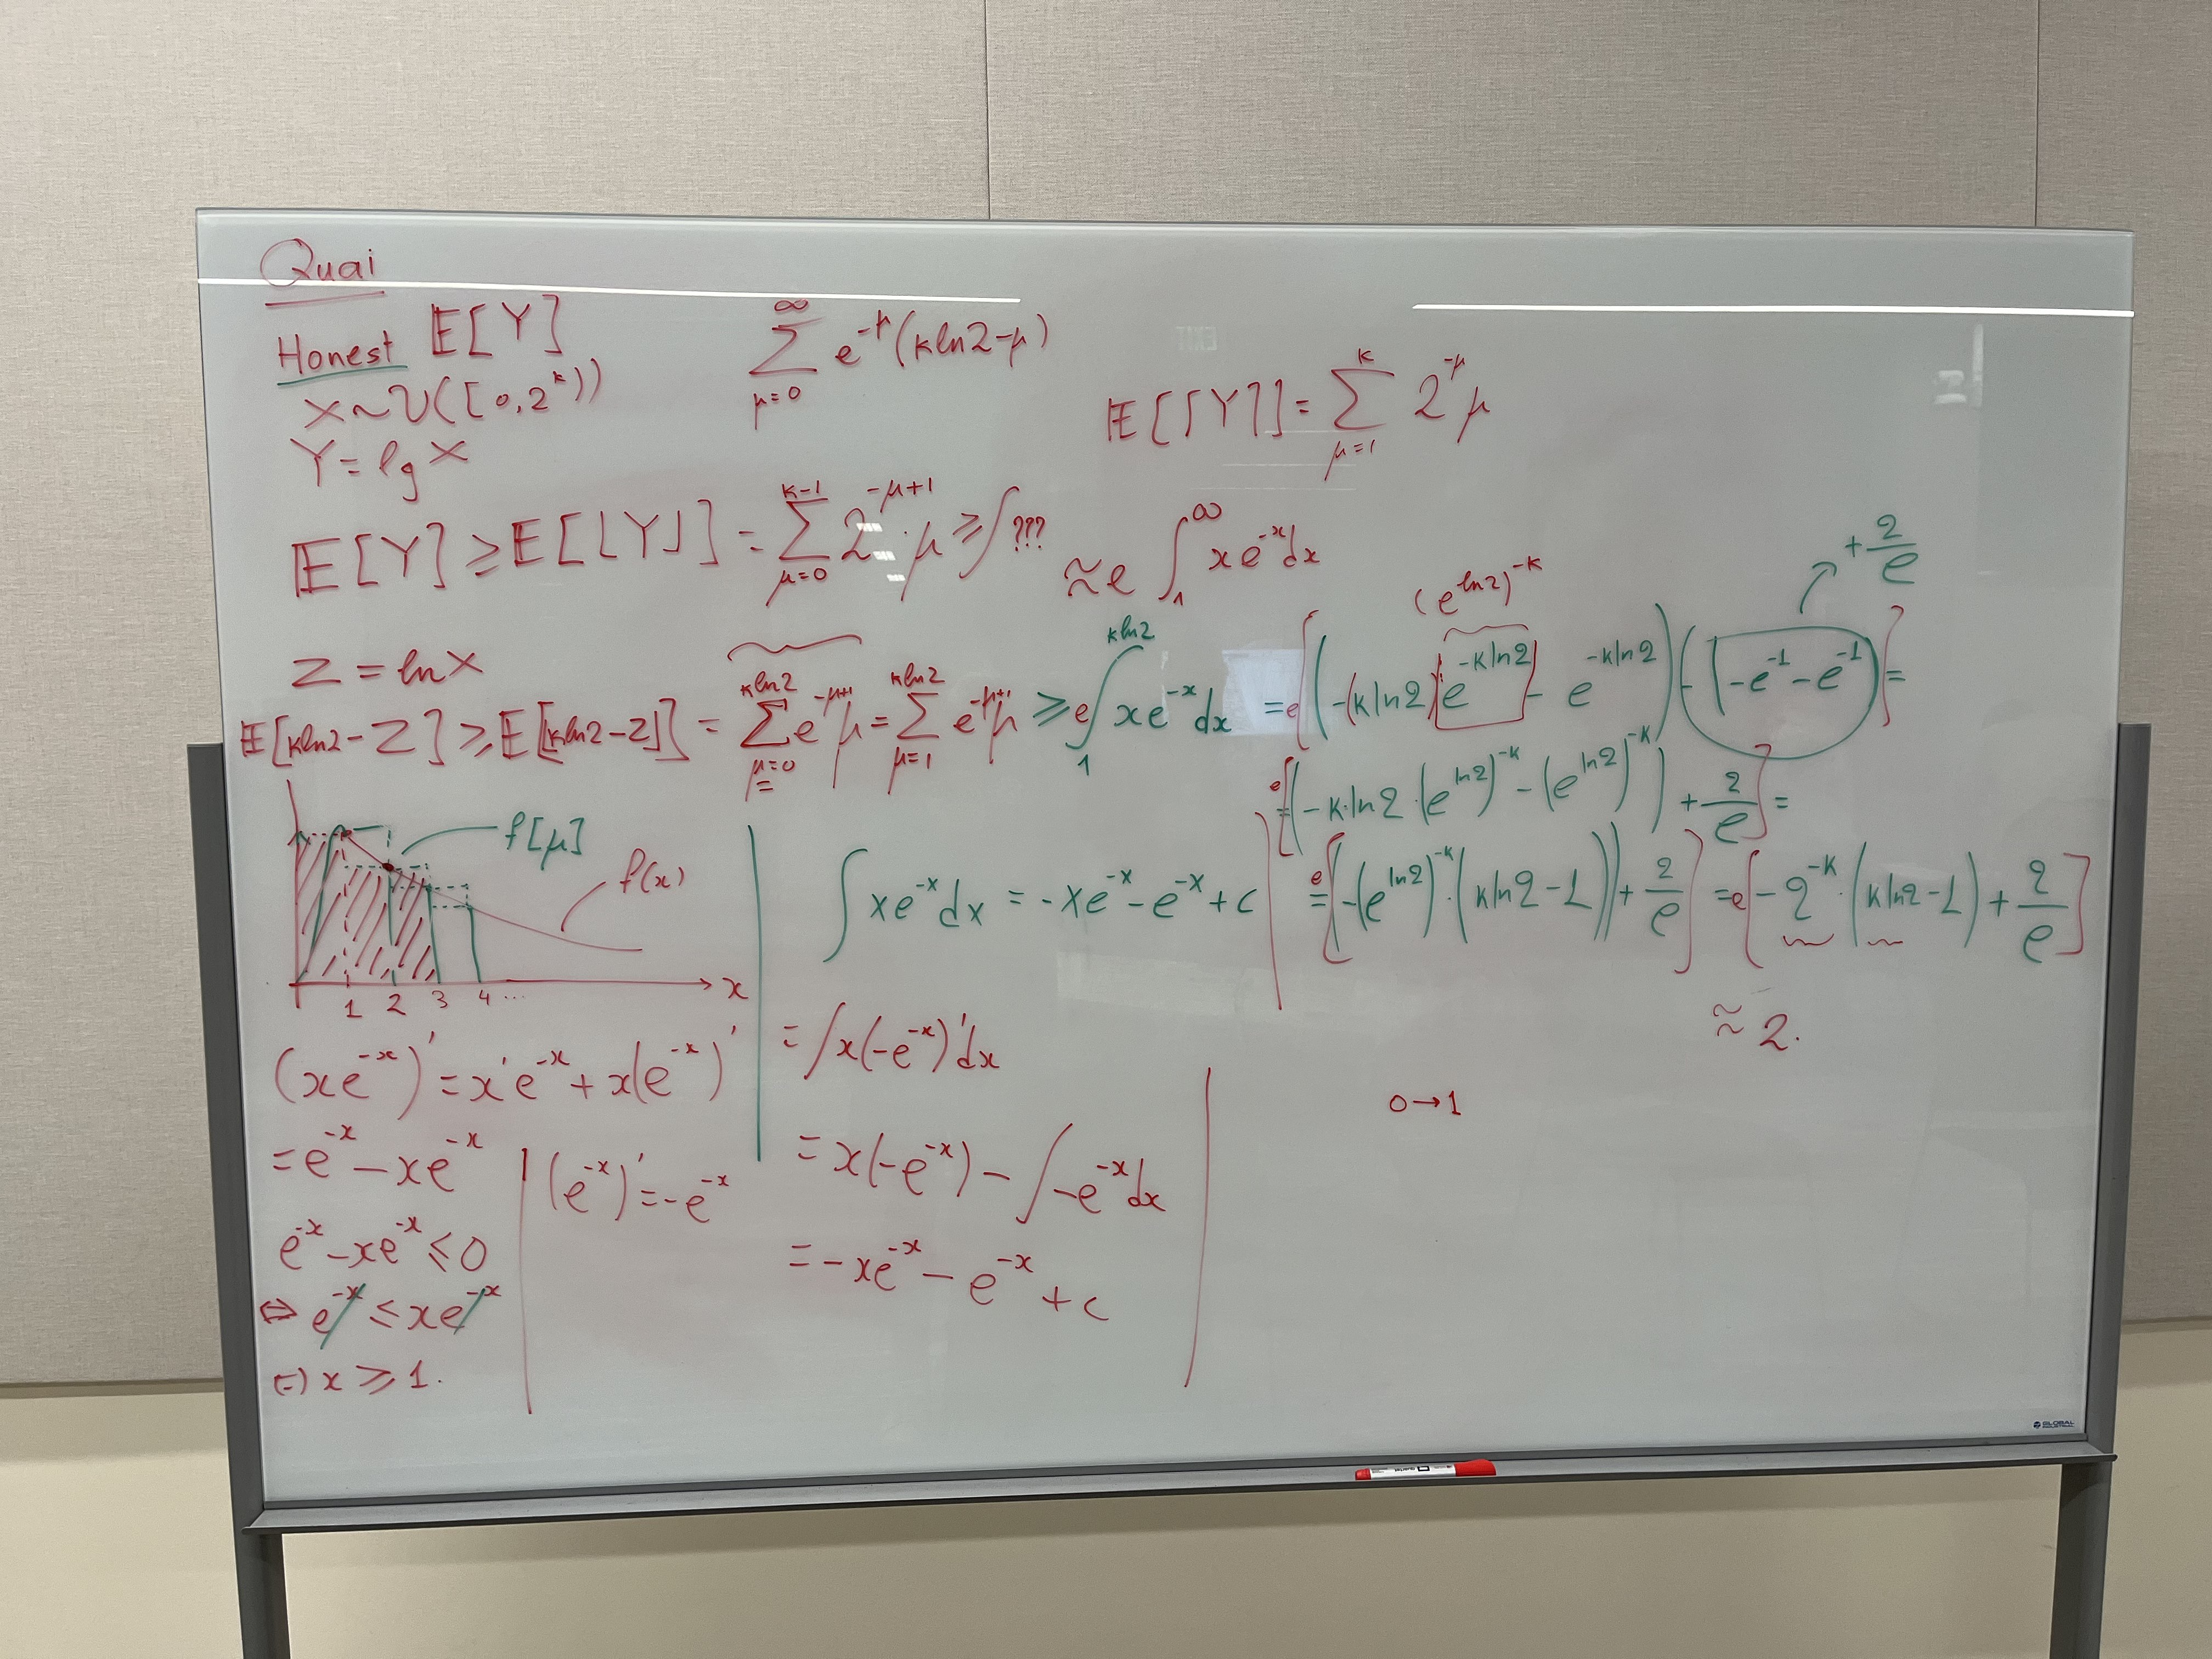
\includegraphics[width=1\textwidth]{figures/bounds-1.jpeg}
\end{figure}

\begin{figure}[h]
    \centering
    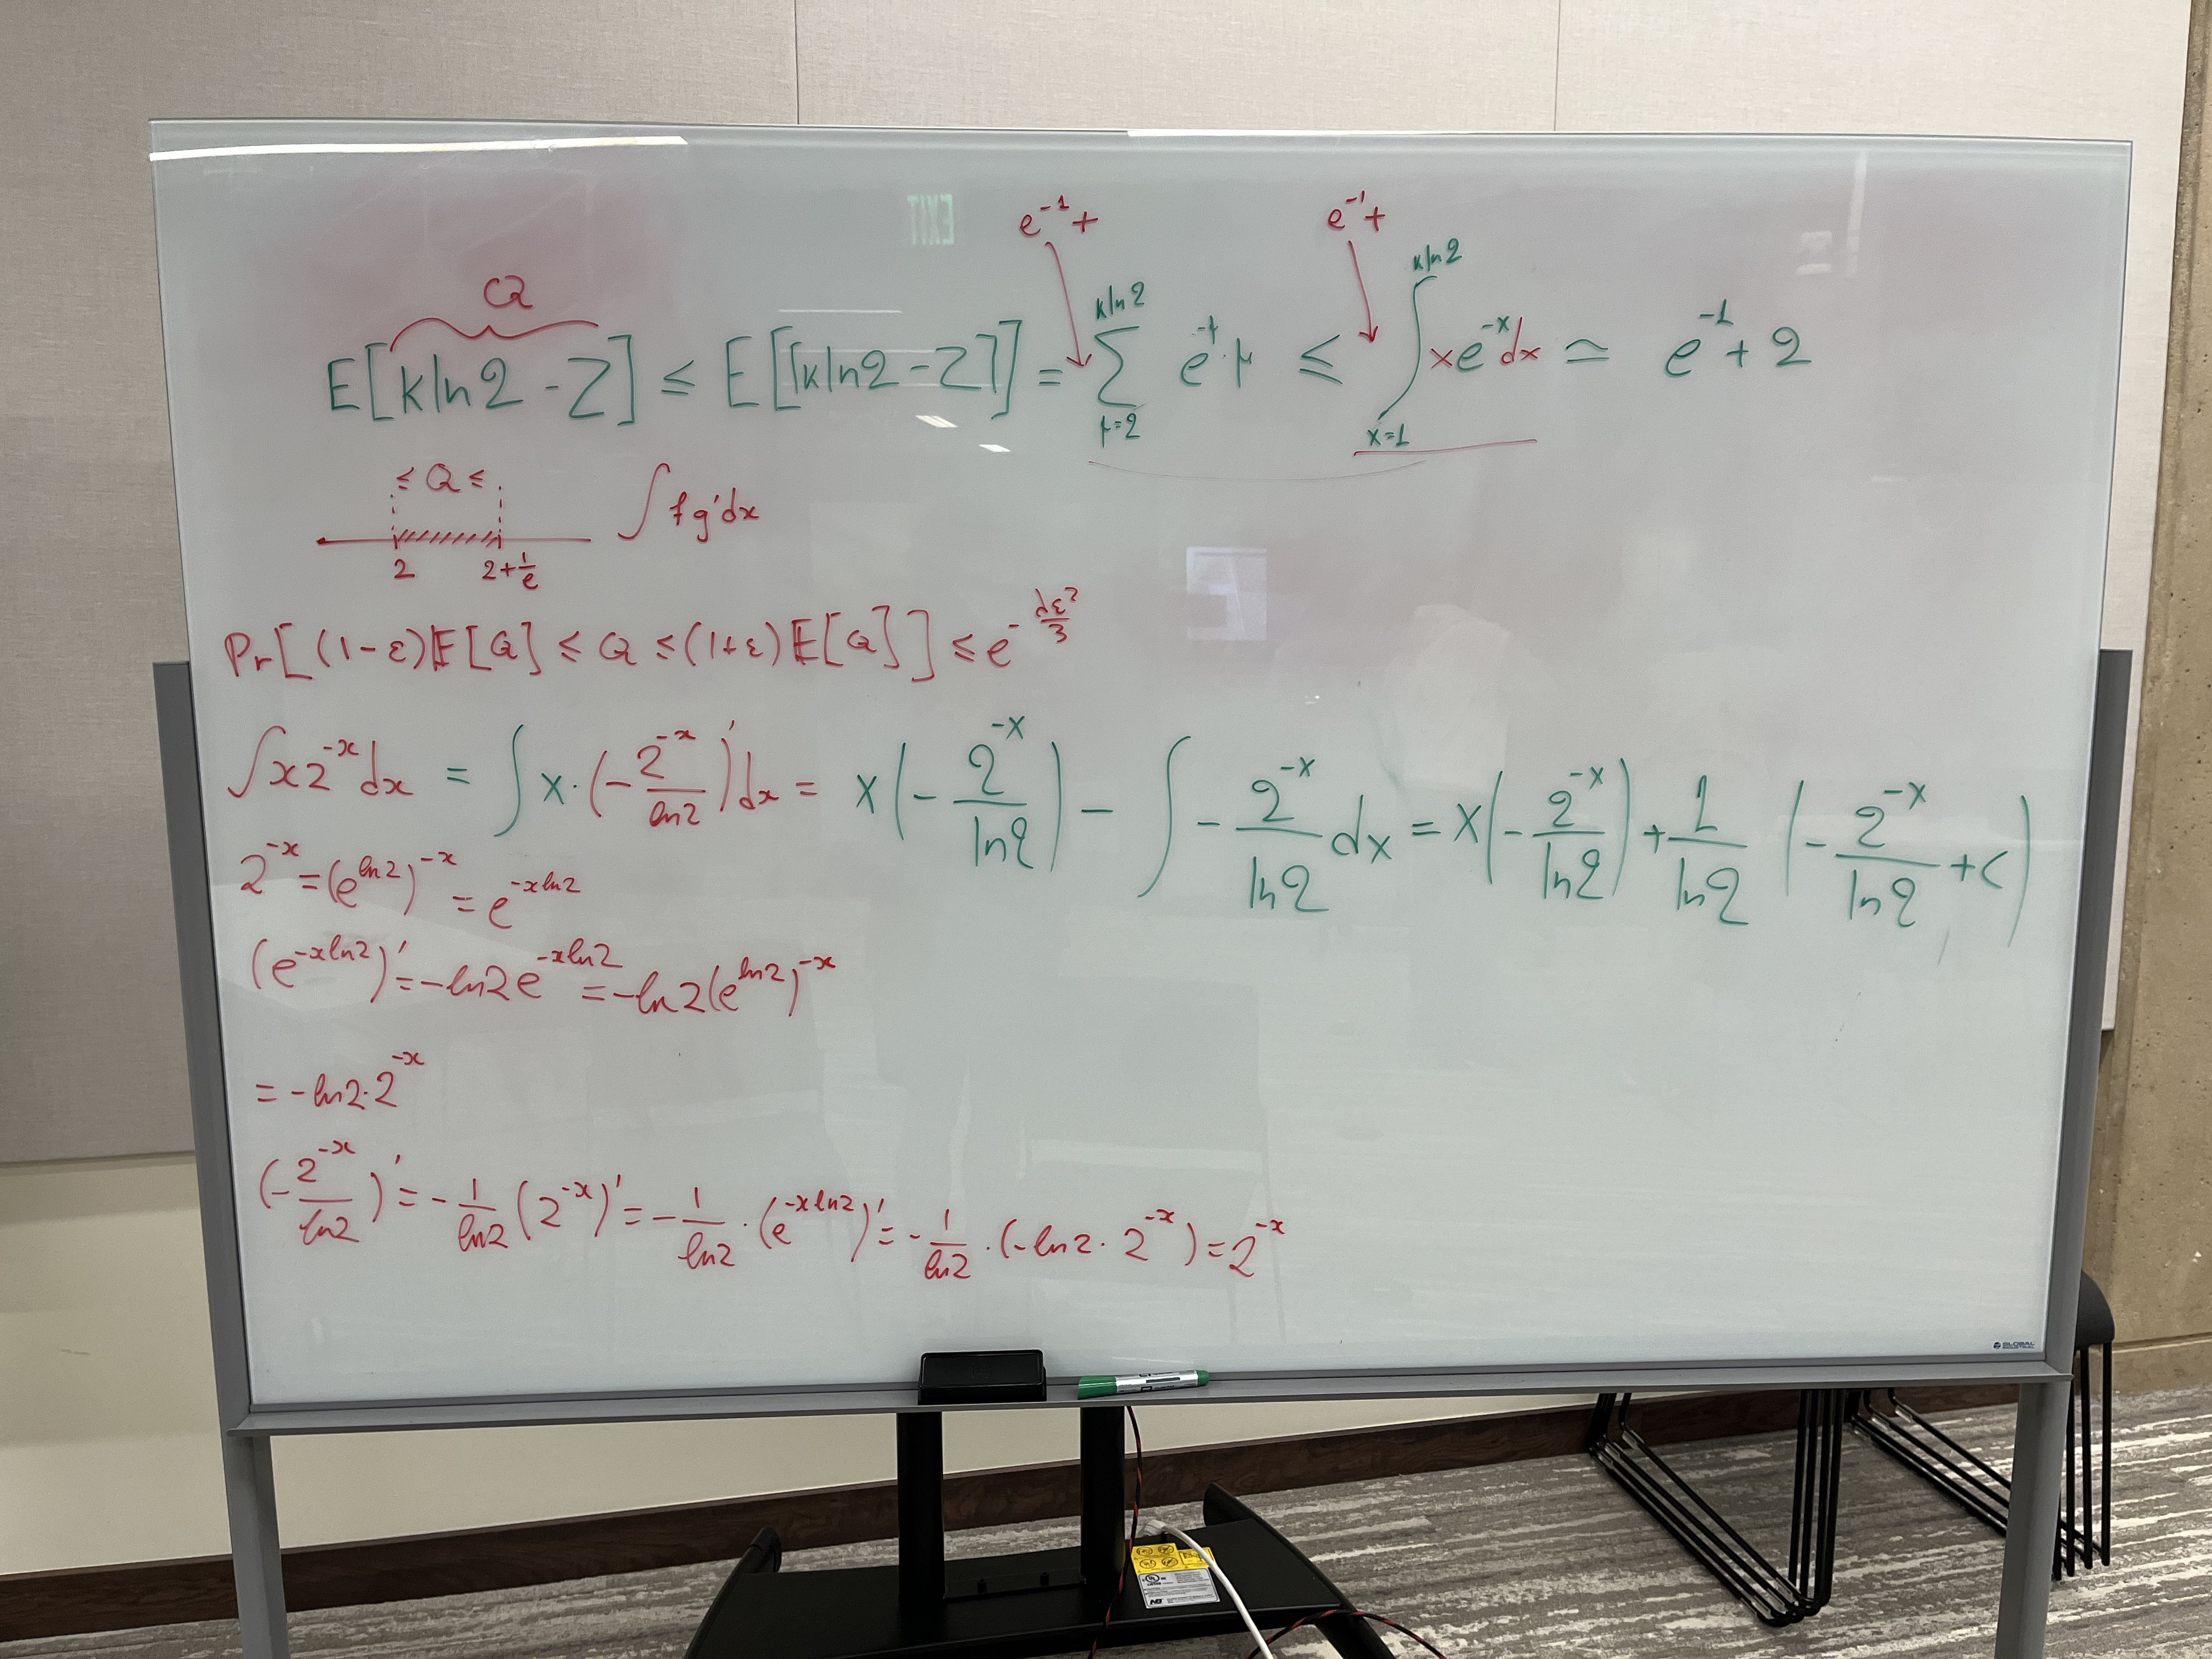
\includegraphics[width=1\textwidth]{figures/bounds-2.jpeg}
\end{figure}
